\documentclass{standalone}
\usepackage{tikz}
\usetikzlibrary{patterns, positioning}


\begin{document}
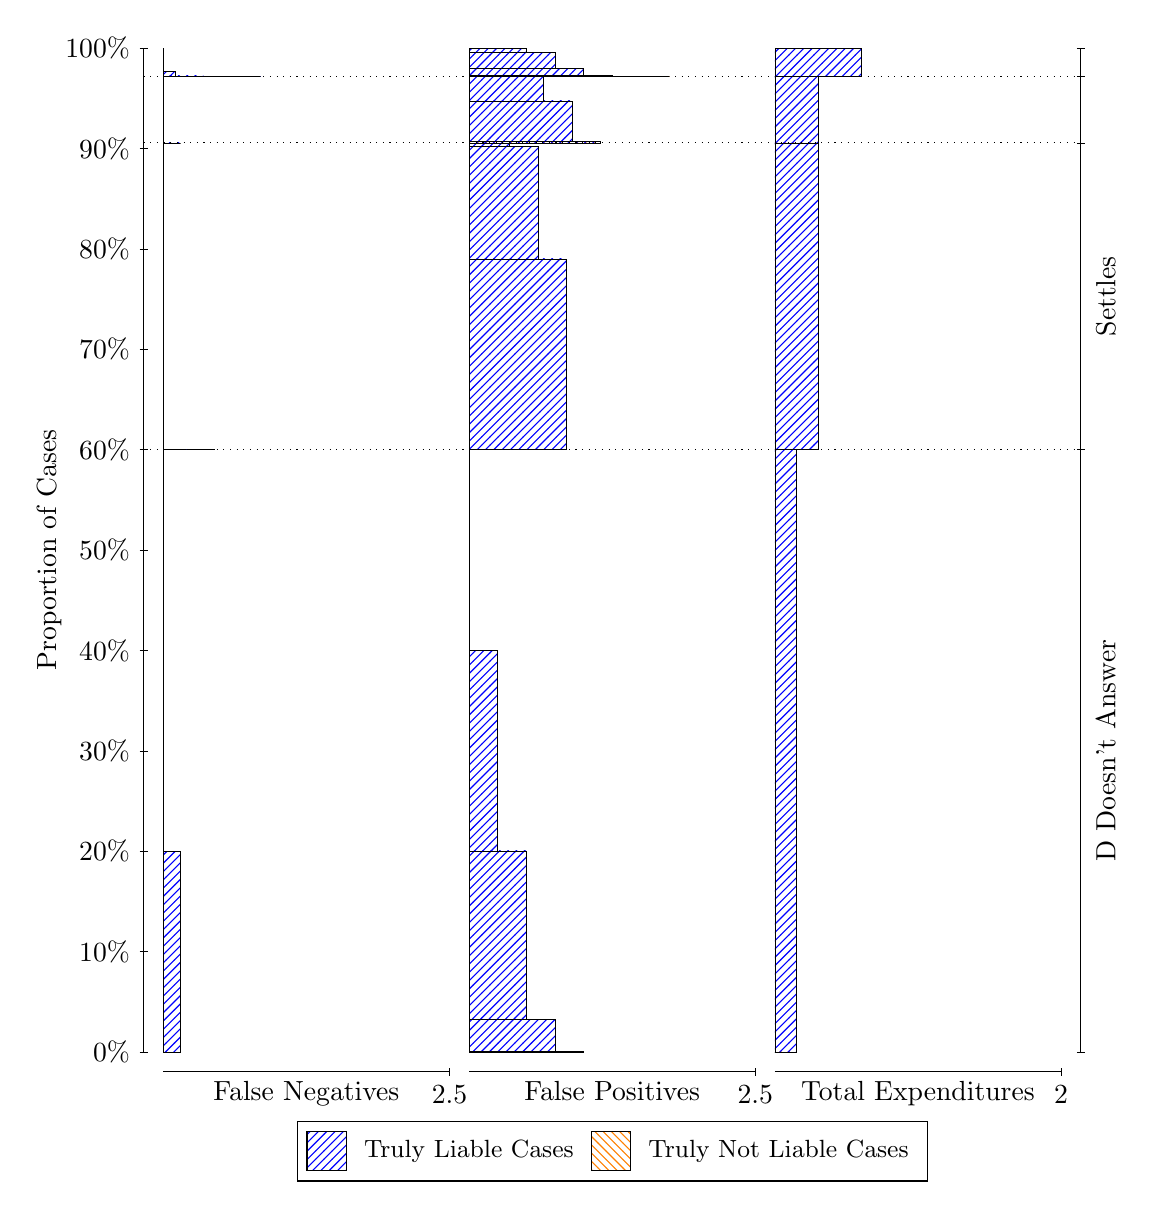
\begin{tikzpicture}
\draw[black, very thin] (1.5,1.75) -- (1.5,14.5);
\node[rotate=90, text=black, anchor=center] at (0.3, 8.125) {Proportion of Cases};
\draw[black, very thin] (1.45,1.75) -- (1.55,1.75);
\node[text=black, anchor=east] at (1.45, 1.75) {0\%};
\draw[black, very thin] (1.45,3.025) -- (1.55,3.025);
\node[text=black, anchor=east] at (1.45, 3.025) {10\%};
\draw[black, very thin] (1.45,4.3) -- (1.55,4.3);
\node[text=black, anchor=east] at (1.45, 4.3) {20\%};
\draw[black, very thin] (1.45,5.575) -- (1.55,5.575);
\node[text=black, anchor=east] at (1.45, 5.575) {30\%};
\draw[black, very thin] (1.45,6.85) -- (1.55,6.85);
\node[text=black, anchor=east] at (1.45, 6.85) {40\%};
\draw[black, very thin] (1.45,8.125) -- (1.55,8.125);
\node[text=black, anchor=east] at (1.45, 8.125) {50\%};
\draw[black, very thin] (1.45,9.4) -- (1.55,9.4);
\node[text=black, anchor=east] at (1.45, 9.4) {60\%};
\draw[black, very thin] (1.45,10.675) -- (1.55,10.675);
\node[text=black, anchor=east] at (1.45, 10.675) {70\%};
\draw[black, very thin] (1.45,11.95) -- (1.55,11.95);
\node[text=black, anchor=east] at (1.45, 11.95) {80\%};
\draw[black, very thin] (1.45,13.225) -- (1.55,13.225);
\node[text=black, anchor=east] at (1.45, 13.225) {90\%};
\draw[black, very thin] (1.45,14.5) -- (1.55,14.5);
\node[text=black, anchor=east] at (1.45, 14.5) {100\%};

\draw[black, very thin] (13.4,1.75) -- (13.4,14.5);
\draw[black, very thin] (13.35,1.75) -- (13.45,1.75);
\node[anchor=west] at (13.35, 1.75) {};
\draw[black, very thin] (13.35,9.4012) -- (13.45,9.4012);
\node[anchor=west] at (13.35, 9.4012) {};
\draw[black, very thin] (13.35,13.296) -- (13.45,13.296);
\node[anchor=west] at (13.35, 13.296) {};
\draw[black, very thin] (13.35,14.144) -- (13.45,14.144);
\node[anchor=west] at (13.35, 14.144) {};
\draw[black, very thin] (13.35,14.5) -- (13.45,14.5);
\node[anchor=west] at (13.35, 14.5) {};

\draw[black, very thin, pattern color=blue, pattern=north east lines] (1.75,1.75) rectangle (1.968,4.2999);
\draw[black, very thin, pattern color=orange, pattern=north west lines] (1.75,4.2999) rectangle (1.75,4.2999);
\draw[black, very thin, pattern color=blue, pattern=north east lines] (1.75,4.2999) rectangle (1.75,9.4012);
\draw[black, very thin, pattern color=blue, pattern=north east lines] (1.75,9.4012) rectangle (2.404,9.4012);
\draw[black, very thin, pattern color=blue, pattern=north east lines] (1.75,9.4012) rectangle (2.0407,9.4012);
\draw[black, very thin, pattern color=orange, pattern=north west lines] (1.75,9.4012) rectangle (1.75,9.4012);
\draw[black, very thin, pattern color=blue, pattern=north east lines] (1.75,9.4012) rectangle (1.75,13.296);
\draw[black, very thin, pattern color=blue, pattern=north east lines] (1.75,13.296) rectangle (1.968,13.296);
\draw[black, very thin, pattern color=orange, pattern=north west lines] (1.75,13.296) rectangle (1.75,13.296);
\draw[black, very thin, pattern color=blue, pattern=north east lines] (1.75,13.296) rectangle (1.75,14.144);
\draw[black, very thin, pattern color=blue, pattern=north east lines] (1.75,14.144) rectangle (2.9853,14.144);
\draw[black, very thin, pattern color=blue, pattern=north east lines] (1.75,14.144) rectangle (2.622,14.144);
\draw[black, very thin, pattern color=blue, pattern=north east lines] (1.75,14.144) rectangle (2.2587,14.144);
\draw[black, very thin, pattern color=blue, pattern=north east lines] (1.75,14.144) rectangle (2.2587,14.145);
\draw[black, very thin, pattern color=blue, pattern=north east lines] (1.75,14.145) rectangle (1.8953,14.145);
\draw[black, very thin, pattern color=blue, pattern=north east lines] (1.75,14.145) rectangle (1.8953,14.204);
\draw[black, very thin, pattern color=orange, pattern=north west lines] (1.75,14.204) rectangle (1.75,14.204);
\draw[black, very thin, pattern color=blue, pattern=north east lines] (1.75,14.204) rectangle (1.75,14.5);
\draw[black, very thin, pattern color=orange, pattern=north west lines] (5.6333,1.75) rectangle (7.0867,1.75);
\draw[black, very thin, pattern color=blue, pattern=north east lines] (5.6333,1.75) rectangle (7.0867,1.7541);
\draw[black, very thin, pattern color=blue, pattern=north east lines] (5.6333,1.7541) rectangle (6.7233,2.1592);
\draw[black, very thin, pattern color=blue, pattern=north east lines] (5.6333,2.1592) rectangle (6.36,4.3047);
\draw[black, very thin, pattern color=blue, pattern=north east lines] (5.6333,4.3047) rectangle (5.9967,6.8512);
\draw[black, very thin, pattern color=blue, pattern=north east lines] (5.6333,6.8512) rectangle (5.6333,9.4012);
\draw[black, very thin, pattern color=orange, pattern=north west lines] (5.6333,9.4012) rectangle (6.8687,9.4012);
\draw[black, very thin, pattern color=blue, pattern=north east lines] (5.6333,9.4012) rectangle (6.8687,11.821);
\draw[black, very thin, pattern color=blue, pattern=north east lines] (5.6333,11.821) rectangle (6.5053,13.248);
\draw[black, very thin, pattern color=blue, pattern=north east lines] (5.6333,13.248) rectangle (6.142,13.296);
\draw[black, very thin, pattern color=blue, pattern=north east lines] (5.6333,13.296) rectangle (5.7787,13.296);
\draw[black, very thin, pattern color=blue, pattern=north east lines] (5.6333,13.296) rectangle (5.6333,13.296);
\draw[black, very thin, pattern color=orange, pattern=north west lines] (5.6333,13.296) rectangle (7.3047,13.296);
\draw[black, very thin, pattern color=blue, pattern=north east lines] (5.6333,13.296) rectangle (7.3047,13.317);
\draw[black, very thin, pattern color=blue, pattern=north east lines] (5.6333,13.317) rectangle (6.9413,13.83);
\draw[black, very thin, pattern color=blue, pattern=north east lines] (5.6333,13.83) rectangle (6.578,14.141);
\draw[black, very thin, pattern color=blue, pattern=north east lines] (5.6333,14.141) rectangle (6.2147,14.144);
\draw[black, very thin, pattern color=blue, pattern=north east lines] (5.6333,14.144) rectangle (5.8513,14.144);
\draw[black, very thin, pattern color=orange, pattern=north west lines] (5.6333,14.144) rectangle (8.1767,14.144);
\draw[black, very thin, pattern color=blue, pattern=north east lines] (5.6333,14.144) rectangle (8.1767,14.144);
\draw[black, very thin, pattern color=orange, pattern=north west lines] (5.6333,14.144) rectangle (7.8133,14.144);
\draw[black, very thin, pattern color=blue, pattern=north east lines] (5.6333,14.144) rectangle (7.8133,14.144);
\draw[black, very thin, pattern color=orange, pattern=north west lines] (5.6333,14.144) rectangle (7.45,14.144);
\draw[black, very thin, pattern color=blue, pattern=north east lines] (5.6333,14.144) rectangle (7.45,14.153);
\draw[black, very thin, pattern color=orange, pattern=north west lines] (5.6333,14.153) rectangle (7.0867,14.153);
\draw[black, very thin, pattern color=blue, pattern=north east lines] (5.6333,14.153) rectangle (7.0867,14.244);
\draw[black, very thin, pattern color=orange, pattern=north west lines] (5.6333,14.244) rectangle (6.7233,14.244);
\draw[black, very thin, pattern color=blue, pattern=north east lines] (5.6333,14.244) rectangle (6.7233,14.44);
\draw[black, very thin, pattern color=blue, pattern=north east lines] (5.6333,14.44) rectangle (6.36,14.499);
\draw[black, very thin, pattern color=blue, pattern=north east lines] (5.6333,14.499) rectangle (5.9967,14.5);
\draw[black, very thin, pattern color=blue, pattern=north east lines] (5.6333,14.5) rectangle (5.6333,14.5);
\draw[black, very thin, pattern color=orange, pattern=north west lines] (9.5167,1.75) rectangle (9.7892,1.75);
\draw[black, very thin, pattern color=blue, pattern=north east lines] (9.5167,1.75) rectangle (9.7892,9.4012);
\draw[black, very thin, pattern color=orange, pattern=north west lines] (9.5167,9.4012) rectangle (10.062,9.4012);
\draw[black, very thin, pattern color=blue, pattern=north east lines] (9.5167,9.4012) rectangle (10.062,13.296);
\draw[black, very thin, pattern color=orange, pattern=north west lines] (9.5167,13.296) rectangle (10.062,13.296);
\draw[black, very thin, pattern color=blue, pattern=north east lines] (9.5167,13.296) rectangle (10.062,14.144);
\draw[black, very thin, pattern color=orange, pattern=north west lines] (9.5167,14.144) rectangle (10.607,14.144);
\draw[black, very thin, pattern color=blue, pattern=north east lines] (9.5167,14.144) rectangle (10.607,14.5);
\draw[black, dotted] (1.5,9.4012) -- (13.4,9.4012);
\draw[black, dotted] (1.5,13.296) -- (13.4,13.296);
\draw[black, dotted] (1.5,14.144) -- (13.4,14.144);
\draw[black, very thin] (1.75,1.5) -- (5.3833,1.5);
\node[text=black, anchor=north] at (3.5667, 1.5) {False Negatives};
\draw[black, very thin] (5.3833,1.45) -- (5.3833,1.55);
\node[text=black, anchor=north] at (5.3833, 1.45) {2.5};

\draw[black, very thin] (5.6333,1.5) -- (9.2667,1.5);
\node[text=black, anchor=north] at (7.45, 1.5) {False Positives};
\draw[black, very thin] (9.2667,1.45) -- (9.2667,1.55);
\node[text=black, anchor=north] at (9.2667, 1.45) {2.5};

\draw[black, very thin] (9.5167,1.5) -- (13.15,1.5);
\node[text=black, anchor=north] at (11.333, 1.5) {Total Expenditures};
\draw[black, very thin] (13.15,1.45) -- (13.15,1.55);
\node[text=black, anchor=north] at (13.15, 1.45) {2};

\node[text=black, centered, rotate=90] at (13.72, 5.5756) {D Doesn't Answer};
\node[text=black, centered, rotate=90] at (13.72, 11.348) {Settles};



\draw (7.449999999999999,1.5) node[draw=none] (baseCoordinate) {};
\begin{scope}[align=center]
        \matrix[scale=0.5, draw=black, below=0.5cm of baseCoordinate, nodes={draw}, column sep=0.1cm]{
            \node[rectangle, draw, minimum width=0.5cm, minimum height=0.5cm, pattern color=blue, pattern=north east lines] {}; &
            \node[draw=none, font=\small, text=black] (B) {Truly Liable Cases}; &
            \node[rectangle, draw, minimum width=0.5cm, minimum height=0.5cm, pattern color=orange, pattern=north west lines] {}; &
            \node[draw=none, font=\small, text=black] (B) {Truly Not Liable Cases}; \\
            };
\end{scope}

\end{tikzpicture}
\end{document}